% FaultLine: supplementary material (review version), compiled separately from main.tex.
\documentclass[10pt,twocolumn,letterpaper]{article}
\usepackage[review]{cvpr}
% Packages and macros used by main.tex and supp.tex (loaded before hyperref).
\usepackage{cuted}      % two-column teaser (strip environment), from the author kit
\usepackage{currfile}
\usepackage{caption}
\usepackage{array}      % ragged-right p columns in the dataset table
\usepackage{multirow}
\usepackage{xspace}

% Text still waiting for results (human check). Must be empty before submission:
% grep -n "\\pending" sec/*.tex
\newcommand{\pending}[1]{{\color{red}[#1]}}

\newcommand{\name}{FaultLine\xspace}
\newcommand{\Sone}{S1\xspace}
\newcommand{\Stwo}{S2\xspace}
\newcommand{\Sthree}{S3\xspace}

\definecolor{cvprblue}{rgb}{0.21,0.49,0.74}
\usepackage[pagebackref,breaklinks,colorlinks,allcolors=cvprblue]{hyperref}
\def\confName{CVPR}
\def\confYear{2027}
\renewcommand{\thesection}{S\arabic{section}}
\renewcommand{\thetable}{S\arabic{table}}
\renewcommand{\thefigure}{S\arabic{figure}}
\title{Do VLMs Know What Is Wrong? A Joint Benchmark of\\Cross-Modal Conflict Detection, Resolution, and Attribution}

\begin{document}
\maketitlesupplementary

This supplement gives the dataset rules (\cref{sec:s-data}), the exact prompts (\cref{sec:s-prompts}), the scoring and parsing rules (\cref{sec:s-parse}), additional results (\cref{sec:s-results}), the cross-platform check (\cref{sec:s-platform}), the human check (\cref{sec:s-human}) and compute details (\cref{sec:s-compute}). Every number is computed by scripts from the stored outputs of one run per model; nothing was re-run selectively. Section, table and figure numbers without ``S'' refer to the main paper.

\section{Dataset details}
\label{sec:s-data}

\paragraph{Vocabulary.} 80 canonical object names in 9 groups (vehicle, animal, food, furniture, tableware, electronics, sports, household, street), with aliases and plurals, and 15 colours. People, hypernym pairs and ambiguous object names are excluded. A far colour edit draws from colours outside the true colour's family and its list of near colours; a near edit uses a colour from that list. A far object edit uses another group, a near edit the same group.

\paragraph{Targets and anchors.} A target is the only instance of its name in the photo and covers at least 2\% of it. An anchor (the reference object of a relation) has a unique name, covers at least 1\%, and is in the vocabulary or one of eight large scene objects (tree, building, window, door, fence, house, plant, flower). Spatial relations are recomputed from the boxes (main paper, Sec.~3); diagonal and overlapping pairs never appear.

\paragraph{Descriptions.} Attribute edits require exactly one colour label on the target, which must not be an animal; the same rule decides when a colour may appear anywhere in a description. Object replacements are absent from the photo under all aliases, the target colour is dropped from object sentences so that implausible combinations do not reveal the edit from the text alone, and no other vocabulary object stands in the same relation to the anchor. A description may contain one faithful filler sentence about another object, placed before or after the target sentence at random.

\paragraph{Allocation.} Candidate supply is uneven: 720 object targets qualify for \Sone against 3,161 attribute targets for \Sthree. Targets are assigned to cells by max--min fair allocation with augmenting paths, filling the main quotas before reserves, with at most two records per image and each object used once. The core set takes 200 records per cell; the release adds the remaining records (4,062 in total; object and relation cells are capped at 379 by the per-image limit).

\section{Prompts}
\label{sec:s-prompts}
% generated by scripts/make_prompt_appendix.py from prompt version p1.1
Prompts for record fl\_00002 (object, S3): the description says ``ball'' where the image shows ``skateboard''. [image] marks where the photo is attached. Multiple-choice probes are scored from the probabilities of the four option letters as the next token; generated probes use greedy decoding.

\paragraph{Image only.} Perception control: the question from the image alone, no description.

\noindent\fbox{\parbox{\dimexpr\linewidth-2\fboxsep-2\fboxrule}{\ttfamily\footnotesize
\textbf{User:} [image] What is below the fence?\newline A. ball\newline B. surfboard\newline C. snowboard\newline D. skateboard\newline Answer with the option's letter from the given choices directly.
}}

\paragraph{Text only.} Reading control: the question from the description alone, no image.

\noindent\fbox{\parbox{\dimexpr\linewidth-2\fboxsep-2\fboxrule}{\ttfamily\footnotesize
\textbf{User:} Description: "The ball is below the fence."\newline What is below the fence?\newline A. ball\newline B. surfboard\newline C. snowboard\newline D. skateboard\newline Answer with the option's letter from the given choices directly.
}}

\paragraph{Detect.} Detection: is the description accurate? (yes/no, then a reason)

\noindent\fbox{\parbox{\dimexpr\linewidth-2\fboxsep-2\fboxrule}{\ttfamily\footnotesize
\textbf{User:} [image] Here is a description of the image: "The ball is below the fence."\newline Does the description accurately describe the image? Answer "yes" or "no" first, then explain briefly.
}}

\paragraph{Open.} Resolution, open-ended answer.

\noindent\fbox{\parbox{\dimexpr\linewidth-2\fboxsep-2\fboxrule}{\ttfamily\footnotesize
\textbf{User:} [image] Description: "The ball is below the fence."\newline What is below the fence? Answer with a single word or short phrase.
}}

\paragraph{Multiple choice.} Resolution, multiple choice (scored from the next-token letter probabilities).

\noindent\fbox{\parbox{\dimexpr\linewidth-2\fboxsep-2\fboxrule}{\ttfamily\footnotesize
\textbf{User:} [image] Description: "The ball is below the fence."\newline What is below the fence?\newline A. ball\newline B. surfboard\newline C. snowboard\newline D. skateboard\newline Answer with the option's letter from the given choices directly.
}}

\paragraph{Focus.} Resolution with an instruction to rely on the image.

\noindent\fbox{\parbox{\dimexpr\linewidth-2\fboxsep-2\fboxrule}{\ttfamily\footnotesize
\textbf{User:} [image] Description: "The ball is below the fence."\newline If the description conflicts with the image, rely on the image.\newline What is below the fence?\newline A. ball\newline B. surfboard\newline C. snowboard\newline D. skateboard\newline Answer with the option's letter from the given choices directly.
}}

\paragraph{Attribute.} Attribution: a five-line error report.

\noindent\fbox{\parbox{\dimexpr\linewidth-2\fboxsep-2\fboxrule}{\ttfamily\footnotesize
\textbf{User:} [image] Here is a description of the image: "The ball is below the fence."\newline Check the description against the image. Reply in exactly this format:\newline Error: yes or no\newline Wrong input: text, image, or none\newline Error type: object, attribute, relation, or none\newline Wrong words: the exact wrong words from the description, or none\newline How obvious: obvious, moderate, subtle, or none
}}

\paragraph{Delay.} Control for verbalize: same turns, the assistant turn is a neutral reply.

\noindent\fbox{\parbox{\dimexpr\linewidth-2\fboxsep-2\fboxrule}{\ttfamily\footnotesize
\textbf{User:} [image] Here is a description of the image: "The ball is below the fence."
\par\smallskip
\textbf{Assistant:} OK.
\par\smallskip
\textbf{User:} What is below the fence?\newline A. ball\newline B. surfboard\newline C. snowboard\newline D. skateboard\newline Answer with the option's letter from the given choices directly.
}}

\paragraph{Check (silent).} Control for verbalize: the check prompt, then a neutral reply.

\noindent\fbox{\parbox{\dimexpr\linewidth-2\fboxsep-2\fboxrule}{\ttfamily\footnotesize
\textbf{User:} [image] Here is a description of the image: "The ball is below the fence."\newline Check the description against the image. Reply in exactly this format:\newline Error: yes or no\newline Wrong input: text, image, or none\newline Error type: object, attribute, relation, or none\newline Wrong words: the exact wrong words from the description, or none\newline How obvious: obvious, moderate, subtle, or none
\par\smallskip
\textbf{Assistant:} OK.
\par\smallskip
\textbf{User:} What is below the fence?\newline A. ball\newline B. surfboard\newline C. snowboard\newline D. skateboard\newline Answer with the option's letter from the given choices directly.
}}

\paragraph{Verbalize.} The model's own error report as the assistant turn, then the question.

\noindent\fbox{\parbox{\dimexpr\linewidth-2\fboxsep-2\fboxrule}{\ttfamily\footnotesize
\textbf{User:} [image] Here is a description of the image: "The ball is below the fence."\newline Check the description against the image. Reply in exactly this format:\newline Error: yes or no\newline Wrong input: text, image, or none\newline Error type: object, attribute, relation, or none\newline Wrong words: the exact wrong words from the description, or none\newline How obvious: obvious, moderate, subtle, or none
\par\smallskip
\textbf{Assistant:} <the model's own reply to the Attribute probe>
\par\smallskip
\textbf{User:} What is below the fence?\newline A. ball\newline B. surfboard\newline C. snowboard\newline D. skateboard\newline Answer with the option's letter from the given choices directly.
}}



\section{Scoring and parsing}
\label{sec:s-parse}

\paragraph{Multiple choice.} We read the next-token distribution after the prompt and take the probability of each option letter (``A'' and `` A'' summed), renormalised over the four letters; the chosen option is the most probable letter.

\paragraph{Detection.} The first ``yes''/``no'' within the first six words, otherwise a short list of phrases; anything else is unparsed and counted as not flagged. No detection answer was unparsed.

\paragraph{Open answers.} Colours, object names (with aliases and plurals) and relations are extracted; an answer is the photo's if only the true value is mentioned, the description's if only the edited value is mentioned, and other otherwise.

\paragraph{Attribution.} The five labelled fields are read leniently (markdown, synonyms such as ``colour'' for attribute and ``description'' for text). Four rules were added after inspecting outputs and before the final analysis; each changes scoring only and was tested on real outputs:
\begin{enumerate}[leftmargin=*,itemsep=1pt]
\item The short label ``Obvious:'' is accepted for ``How obvious:''.
\item Only the named words count for the span: the first quoted segment, or the text before an explanation.
\item A reply of exactly five unlabelled lines is read by position (Qwen3-VL-2B often answers this way).
\item A field that copies the option list (\eg ``Wrong input: text, image, or none'') is no answer; before this rule its first word was scored as the answer. It changed 1,190 fields for Qwen3-VL-2B, 387 for InternVL3-2B, 1,665 for SmolVLM2 and 42 for Qwen2.5-VL-7B; every changed value was checked to be a copied list.
\end{enumerate}

\section{Additional results}
\label{sec:s-results}

\begin{table}[h]
\centering
\scriptsize
\setlength{\tabcolsep}{2.5pt}
\resizebox{\linewidth}{!}{\begin{tabular}{lcccc|ccc}
\toprule
 & \multicolumn{4}{c|}{Answers from the image (\%)} & \multicolumn{3}{c}{Gain (points)} \\
Model & Direct & Delay & Check & Verbalize & Structure & Check & Report \\
\midrule
Qwen3-VL-2B & 39.4 & 27.9 & 26.3 & 37.1 & $-$11.6$^{\ast}$ & $-$1.6 & +10.8$^{\ast}$ \\
Qwen3-VL-4B & 41.3 & 69.8 & 71.9 & 80.0 & +28.6$^{\ast}$ & +2.1$^{\ast}$ & +8.1$^{\ast}$ \\
Qwen3-VL-8B & 54.3 & 69.3 & 78.4 & 82.8 & +15.0$^{\ast}$ & +9.1$^{\ast}$ & +4.4$^{\ast}$ \\
Qwen3-VL-30B-A3B & 59.0 & 63.0 & 64.3 & 78.8 & +4.0$^{\ast}$ & +1.3 & +14.5$^{\ast}$ \\
Qwen3-VL-32B & 43.1 & 64.3 & 79.2 & 85.9 & +21.2$^{\ast}$ & +14.9$^{\ast}$ & +6.7$^{\ast}$ \\
\midrule
Qwen2.5-VL-3B & 18.9 & 24.8 & 20.3 & 23.4 & +5.9$^{\ast}$ & $-$4.6$^{\ast}$ & +3.2$^{\ast}$ \\
Qwen2.5-VL-7B & 65.0 & 71.1 & 75.2 & 80.6 & +6.1$^{\ast}$ & +4.1$^{\ast}$ & +5.4$^{\ast}$ \\
Qwen2.5-VL-32B & 48.8 & 70.6 & 77.4 & 82.0 & +21.8$^{\ast}$ & +6.8$^{\ast}$ & +4.6$^{\ast}$ \\
\midrule
InternVL3-2B & 16.9 & 30.9 & 39.8 & 52.9 & +14.0$^{\ast}$ & +8.9$^{\ast}$ & +13.1$^{\ast}$ \\
InternVL3-8B & 49.4 & 74.3 & 75.5 & 75.2 & +24.8$^{\ast}$ & +1.2 & $-$0.3 \\
\midrule
SmolVLM2-2.2B & 7.8 & 13.7 & 18.1 & 13.3 & +5.8$^{\ast}$ & +4.4$^{\ast}$ & $-$4.7$^{\ast}$ \\
\bottomrule
\end{tabular}
}
\caption{\textbf{Where the verbalize gain comes from.} Answers from the image under the direct question, the delayed question, the check prompt and the model's own report; gains are delay minus direct (structure), check minus delay (being asked to check) and verbalize minus check (the report). $^\ast$: exact McNemar $p<0.001$.}
\label{tab:s-probes}
\end{table}

\begin{table}[h]
\centering
\small
\begin{tabular}{lcc}
\toprule
Conflict type & Detection & Resolution \\
\midrule
Attribute & +13.3 [+8.1, +18.2] & +19.0 [+12.7, +25.4] \\
Object & +5.3 [+3.3, +7.4] & $-$0.8 [$-$6.4, +4.7] \\
Relation & +4.5 [+1.9, +7.2] & +9.6 [+4.3, +15.0] \\
\midrule
All & +7.7 [+5.6, +9.8] & +9.3 [+5.7, +12.7] \\
\bottomrule
\end{tabular}

\caption{\textbf{Severity effect}, \Sone minus \Sthree, pooled over the eleven models (points, 95\% image-clustered interval).}
\label{tab:s-severity}
\end{table}

\begin{figure}[h]
\centering
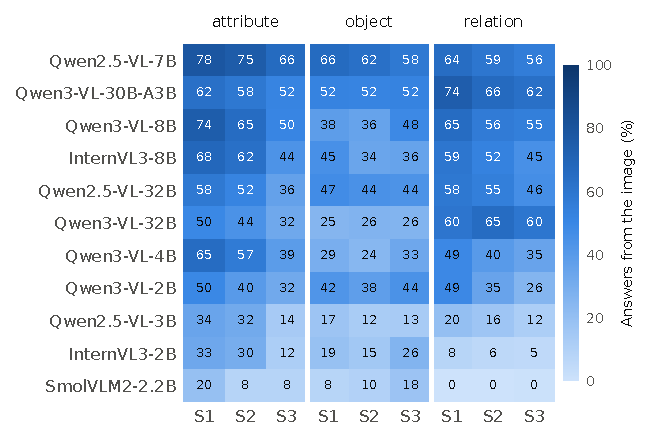
\includegraphics[width=\linewidth]{figures/cells.pdf}
\caption{\textbf{Answers from the image per cell} (\%), models sorted by overall resolution.}
\label{fig:s-cells}
\end{figure}

\begin{table*}[t]
\centering
\scriptsize
\begin{tabular}{lccccccccc}
\toprule
 & \multicolumn{3}{c}{Attribute} & \multicolumn{3}{c}{Object} & \multicolumn{3}{c}{Relation} \\
\cmidrule(lr){2-4}\cmidrule(lr){5-7}\cmidrule(lr){8-10}
Model & S1 & S2 & S3 & S1 & S2 & S3 & S1 & S2 & S3 \\
\midrule
Qwen3-VL-2B & 88/89/50 & 84/85/40 & 88/62/32 & 93/91/42 & 96/84/38 & 92/72/44 & 62/71/49 & 50/73/35 & 47/60/26 \\
Qwen3-VL-4B & 88/92/65 & 89/96/57 & 86/82/39 & 95/100/29 & 95/100/24 & 92/96/33 & 76/98/49 & 68/96/40 & 60/94/35 \\
Qwen3-VL-8B & 88/96/74 & 88/96/65 & 84/85/50 & 94/100/38 & 93/100/36 & 92/97/48 & 73/98/65 & 68/100/56 & 61/96/55 \\
Qwen3-VL-30B-A3B & 88/94/62 & 88/94/58 & 84/81/52 & 94/98/52 & 93/98/52 & 92/98/52 & 74/99/74 & 66/99/66 & 60/95/62 \\
Qwen3-VL-32B & 88/97/50 & 87/99/44 & 87/88/32 & 94/99/25 & 92/99/26 & 92/98/26 & 81/99/60 & 75/100/65 & 74/99/60 \\
\midrule
Qwen2.5-VL-3B & 87/94/34 & 84/94/32 & 85/79/14 & 92/99/17 & 94/100/12 & 93/96/13 & 62/98/20 & 48/96/16 & 46/94/12 \\
Qwen2.5-VL-7B & 86/98/78 & 86/99/75 & 84/92/66 & 93/100/66 & 92/100/62 & 92/99/58 & 72/100/64 & 56/98/59 & 55/98/56 \\
Qwen2.5-VL-32B & 85/92/58 & 84/92/52 & 81/79/36 & 94/99/47 & 94/98/44 & 91/94/44 & 77/98/58 & 69/96/55 & 66/97/46 \\
\midrule
InternVL3-2B & 86/90/33 & 87/88/30 & 82/68/12 & 94/98/19 & 95/92/15 & 93/83/26 & 53/44/8 & 41/48/6 & 31/36/5 \\
InternVL3-8B & 87/93/68 & 86/94/62 & 84/82/44 & 93/99/45 & 93/95/34 & 94/95/36 & 74/98/59 & 68/96/52 & 60/93/45 \\
\midrule
SmolVLM2-2.2B & 86/94/20 & 82/97/8 & 77/88/8 & 88/96/8 & 92/94/10 & 86/92/18 & 38/70/0 & 35/66/0 & 34/62/0 \\
\bottomrule
\end{tabular}

\caption{\textbf{Per cell:} perceive / detect / resolve (\%) for every model, 200 conflicts per cell.}
\label{tab:s-cells}
\end{table*}

\paragraph{Answer position.} The photo's answer is option A/B/C/D in 473/451/440/436 conflicts and the description's in 420/454/444/482. Models pick the photo's answer less often when it is option A (Qwen3-VL-32B: 32\% at A, 45--50\% at B--D), a position bias that averages out over the balanced positions.

\section{Cross-platform check}
\label{sec:s-platform}
The four smallest models were also run in float16 on an Apple-silicon machine (16\,GB, PyTorch MPS) with the same code, prompts and images. \Cref{tab:s-platform} compares the two runs on the same 2,001 records.

\begin{table}[h]
\centering
\scriptsize
\setlength{\tabcolsep}{3pt}
\resizebox{\linewidth}{!}{\begin{tabular}{lcccccc}
\toprule
 & \multicolumn{4}{c}{Identical outputs (\%)} & \multicolumn{2}{c}{Metric change (points)} \\
Model & MC letter & Verbalize & Detection & Error type & $\Delta$ Det. & $\Delta$ Res. \\
\midrule
InternVL3-2B & 99.0 & 95.8 & 98.8 & 93.0 & +0.9 & +0.6 \\
Qwen2.5-VL-3B & 98.7 & 99.2 & 99.2 & 96.0 & $-$0.7 & +0.8 \\
Qwen3-VL-4B & 99.0 & 99.0 & 99.9 & 99.1 & $-$0.6 & +0.2 \\
SmolVLM2-2.2B & 99.5 & 98.3 & 98.7 & 99.5 & $-$0.4 & $-$0.3 \\
\bottomrule
\end{tabular}
}
\caption{\textbf{Same models, two platforms}: Apple silicon float16 vs.\ NVIDIA bfloat16. Identical outputs (\%) and change in headline metrics (points). InternVL3-2B's verbalize controls ran in a separate pass on the first platform.}
\label{tab:s-platform}
\end{table}

\section{Human check}
\label{sec:s-human}
\paragraph{Protocol.} 500 core records (50 per conflict cell, 50 controls split 17/17/16 over question types), all within the first 1,000 records of the stratified order, shown in a fixed random order without cell labels. Per record the annotator (1) answers the multiple-choice question from the photo alone, with ``Can't tell'' for undecidable questions or more than one true option; (2) judges whether the description matches the photo; (3) if not, rates how obvious the mismatch is. Left/right/above/below are as seen in the photo.
\paragraph{Results.} \pending{Per-cell accuracy, valid rate, Cohen's kappa, Spearman correlation of severity with rated obviousness; records both annotators reject.}

\section{Compute and reproducibility}
\label{sec:s-compute}
All reported runs used one NVIDIA DGX Spark (GB10, 128\,GB unified memory) with PyTorch 2.14.1 (CUDA 13.0) and Transformers 5.22.0, bfloat16 and greedy decoding. Measured time per record (all ten probes) ranged from 1.3\,s (Qwen3-VL-2B) to 26.7\,s (Qwen2.5-VL-32B); the eleven models took about 58 GPU-hours in total. The release contains the dataset, the code, every model's raw outputs and the scripts that produce every table and figure.
\end{document}
